\chapter{METHODOLOGY}

The development of our decentralized microblogging platform for scientific communication followed an Agile methodology, prioritizing iterative progress, flexibility, and team collaboration. This chapter outlines the key phases—Requirement Analysis, System Design, Development, Integration with Decentralized Protocols, and Testing—highlighting the processes and strategies that shaped the platform’s realization.

\section{Requirement Analysis}
\label{sec:requirements}

We began by identifying user needs and system requirements through a review of online academic forums, existing social media platforms, and federated system documentation. This research informed essential features: secure data sharing, privacy controls, scientific typesetting support, and decentralized communication. By analyzing the strengths and weaknesses of comparable platforms, we established core functionalities such as user profiles, microblog posts, and cross-instance federation.

\section{Development}
\label{sec:development}

\begin{figure}[h!]
    \centering
    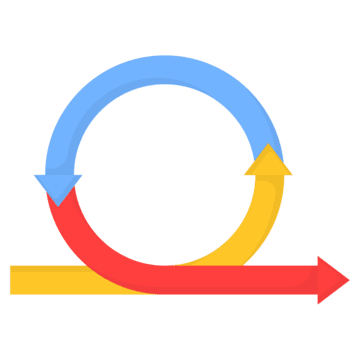
\includegraphics[width=0.5\textwidth]{Graphics/agile.png}
    \caption{Agile Model}
\end{figure}

Development proceeded in iterative Agile sprints, split into backend and frontend streams. This approach allowed continuous refinement based on emerging technical needs and team feedback. The backend handled authentication, content management, and federation, while the frontend focused on delivering an intuitive interface for scientific content creation and consumption.

\section{System Architecture}
 The design phase centered on creating a scalable, federated architecture. We chose the ActivityPub protocol to enable decentralization, structuring the system around a backend for core logic and a mobile-first frontend for user interaction. Emphasis was placed on secure data exchange and usability across devices, with RESTful APIs as the backbone of component communication.

 A modular architecture is used for scalability and maintainability. The figure below gives a high-level view of the system architecture.
\begin{figure}[h!]
    \centering
    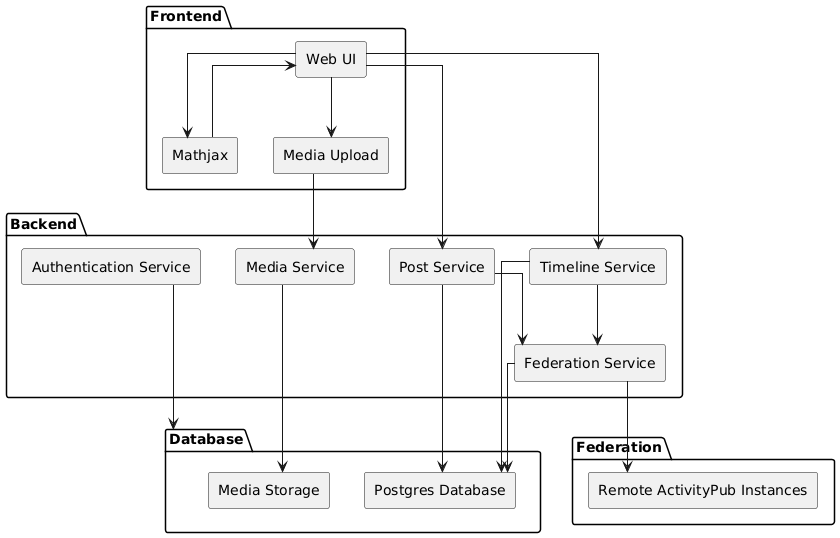
\includegraphics[width=0.8\textwidth]{Graphics/componentdiagram.png}
    \caption{Component Diagram}
\end{figure}

\section{Integration with Decentralized Protocols}
\label{sec:integration}

Federation was a cornerstone of the platform, achieved through ActivityPub compliance. We implemented server-to-server communication and user activity management (e.g., posting, following) to ensure interoperability with other federated systems. This phase was validated iteratively to confirm seamless cross-platform interaction.

\section{Testing}
\label{sec:testing}

Testing was integrated throughout development to maintain functionality and reliability. We employed a multi-layered strategy, including unit tests for individual components and integration tests for system-wide interactions, ensuring robustness at every stage.

\section{Technology Stack and Environment Setup}
\subsection{Backend}
\begin{itemize}
    \item \textbf{Language:} Node.js and Hono Server
    \item \textbf{Database:} Posgres, S3 Storage, Minio
    \item \textbf{Authentication:} OAuth
\end{itemize}

\subsection{Frontend}
\begin{itemize}
    \item \textbf{Framework:} ReactNative, Expo, Mathjax
\end{itemize}

\subsection{Environment}
\begin{itemize}
    \item \textbf{Deployment:} Docker
    \item \textbf{Development:} Docker and Nix
\end{itemize}

\section{Detailed Implementation Steps}
\subsection{Backend Implementation}
\begin{itemize}
    \item \textbf{User Authentication:} Using OAuth.
    \item \textbf{Content Management:} CRUD operations for posts, comments, and likes.
\end{itemize}

\begin{figure}[h!]
    \centering
    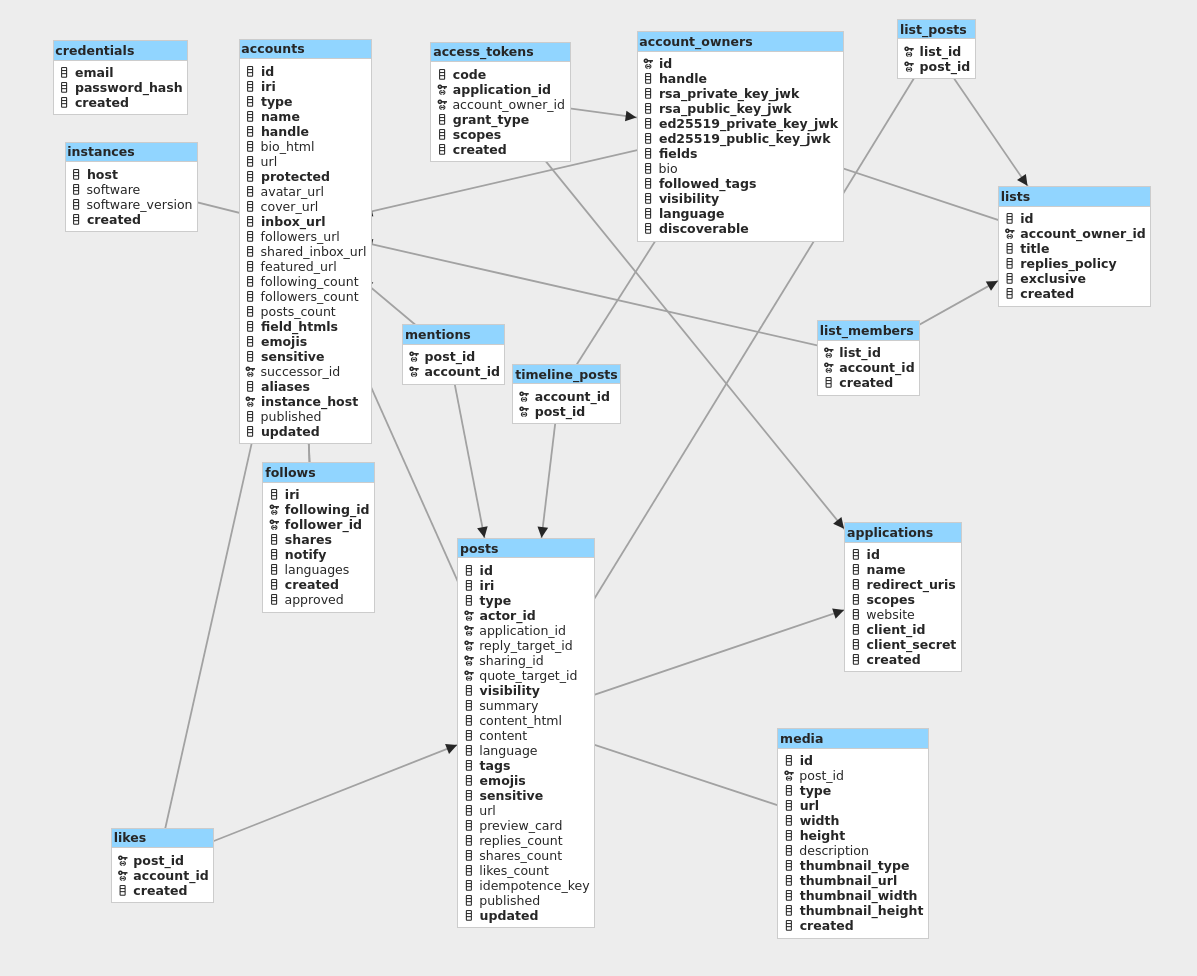
\includegraphics[width=0.8\textwidth]{Graphics/erdiagram.png}
    \caption{ER Diagram}
\end{figure}

\subsection{Frontend Implementation}
\begin{itemize}
    \item \textbf{User Interface:} Developed as a Single-Page Application (SPA) using React.
    \item \textbf{State Management:} Handled with Redux integrating with backend APIs.
\end{itemize}

\section{Use Case}
Integration was performed using API gateways and containerization. Figure \ref{fig:integration} shows the integration flow.
\begin{figure}[h!]
    \centering
    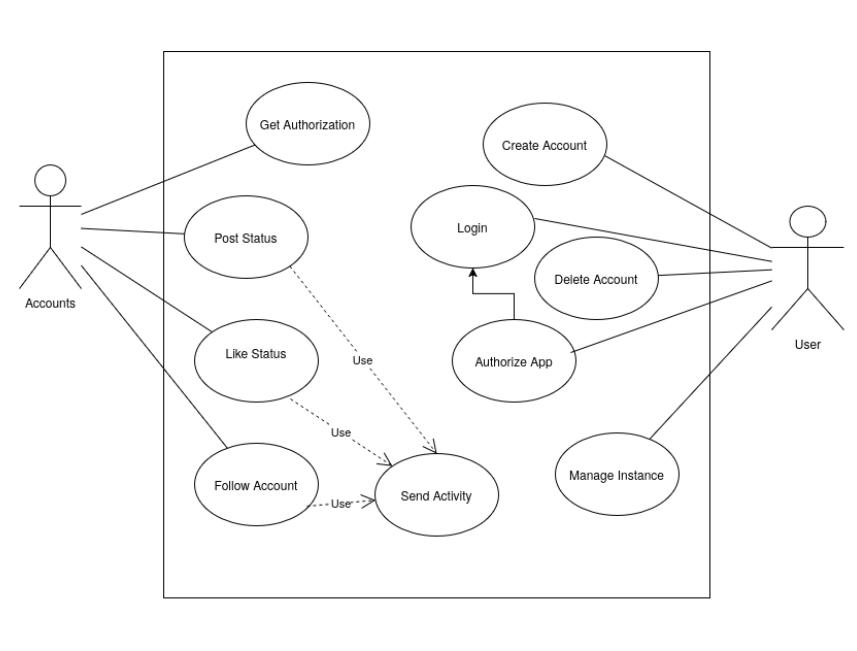
\includegraphics[width=0.8\textwidth]{Graphics/usecasediagram.png}
    \caption{Use Case Diagram}
\end{figure}

